% Appendix A

\chapter{Evaluación de Transcripciones} % Main appendix title

\label{AppendixA} % For referencing this appendix elsewhere, use \ref{AppendixA}

Aquí puede consultar todas las respuestas obtenidas de la encuesta realizada a los contribuyentes donde éstos evaluaban la adecuación de la transcripción con respecto a lenguaje de entrada (source).

\begin{figure}[H]
\centering
	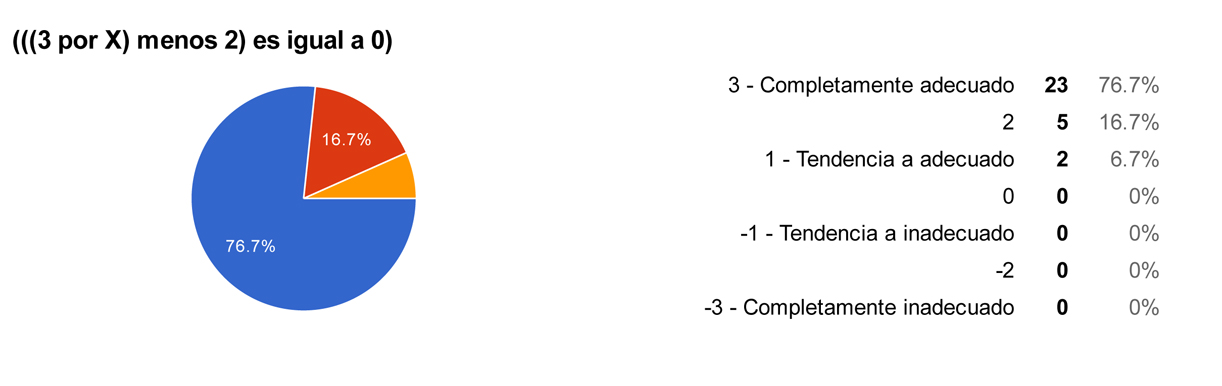
\includegraphics[width=15cm, height=4.74cm]{Figures/hjudgement/r1}
	\caption[]{}
\label{fig:parsed_corpus}
\end{figure}

\begin{figure}[H]
\centering
	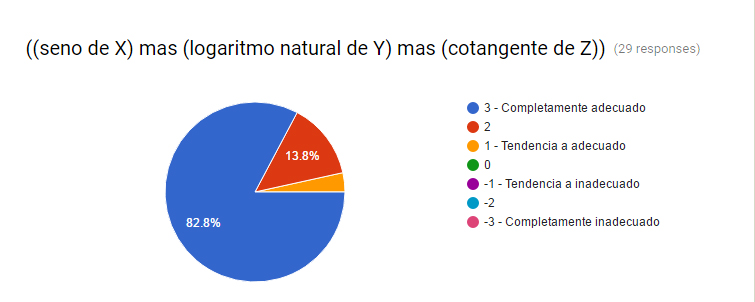
\includegraphics[width=15cm, height=4.74cm]{Figures/hjudgement/r2}
	\caption[]{}
\label{fig:parsed_corpus}
\end{figure}

\begin{figure}[H]
\centering
	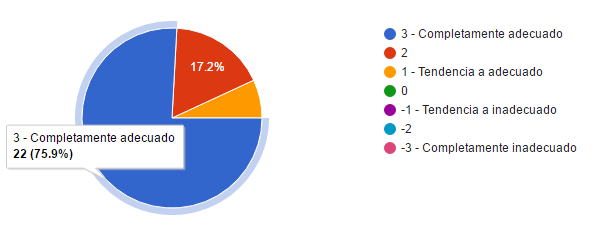
\includegraphics[width=15cm, height=4.74cm]{Figures/hjudgement/r3}
	\caption[]{}
\label{fig:parsed_corpus}
\end{figure}

\begin{figure}[H]
\centering
	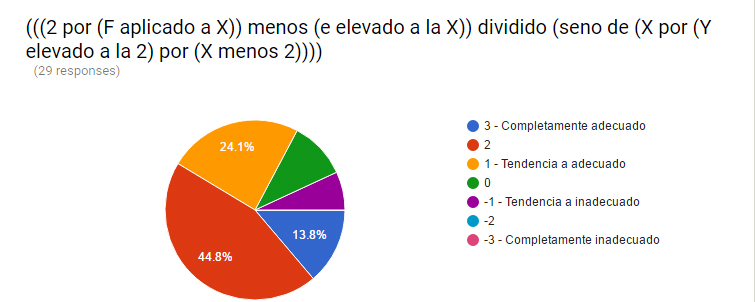
\includegraphics[width=15cm, height=4.74cm]{Figures/hjudgement/r4}
	\caption[]{}
\label{fig:parsed_corpus}
\end{figure}

\begin{figure}[H]
\centering
	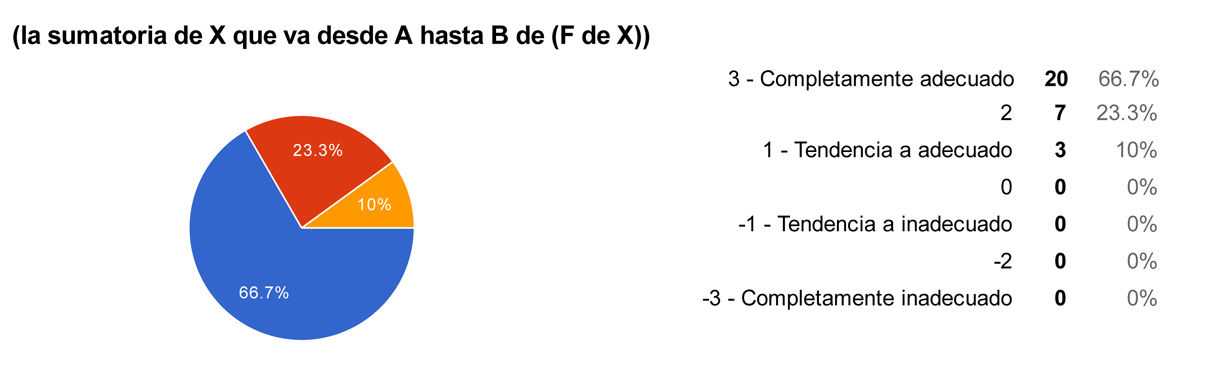
\includegraphics[width=15cm, height=4.74cm]{Figures/hjudgement/r5}
	\caption[]{}
\label{fig:parsed_corpus}
\end{figure}

\begin{figure}[H]
\centering
	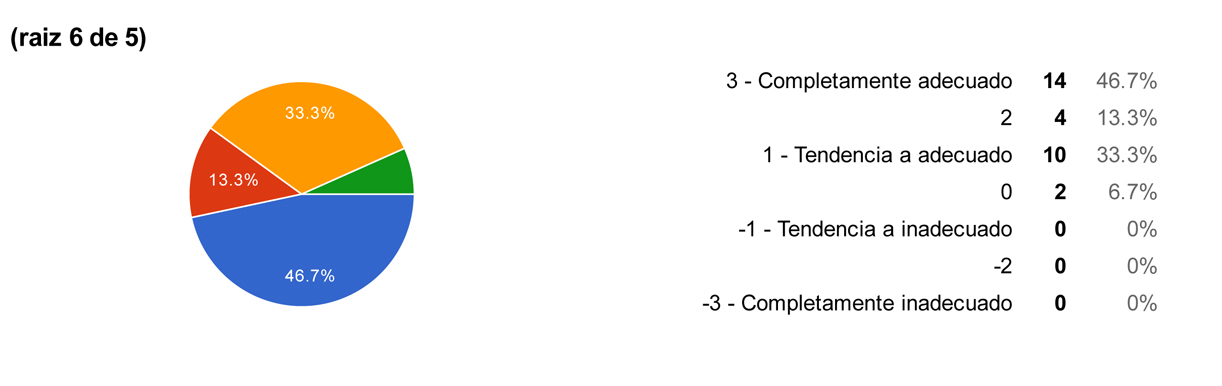
\includegraphics[width=15cm, height=4.74cm]{Figures/hjudgement/r6}
	\caption[]{}
\label{fig:parsed_corpus}
\end{figure}

\begin{figure}[H]
\centering
	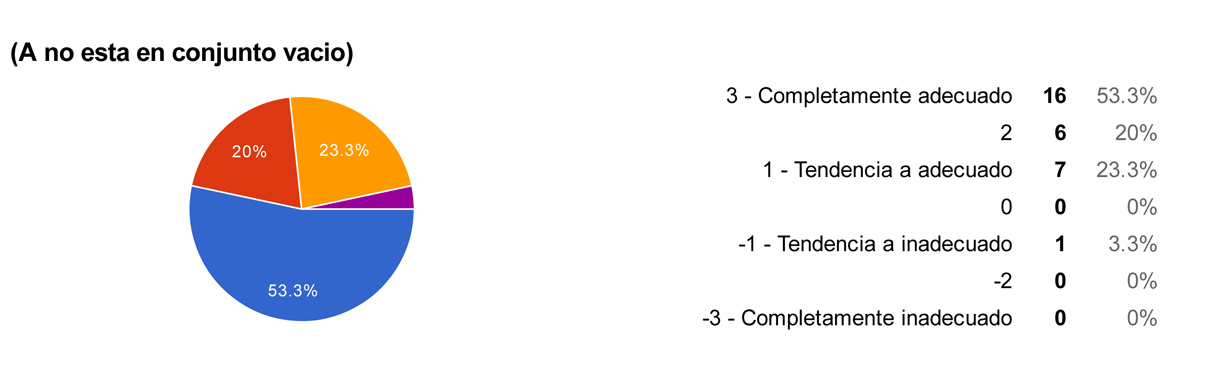
\includegraphics[width=15cm, height=4.74cm]{Figures/hjudgement/r7}
	\caption[]{}
\label{fig:parsed_corpus}
\end{figure}

\begin{figure}[H]
\centering
	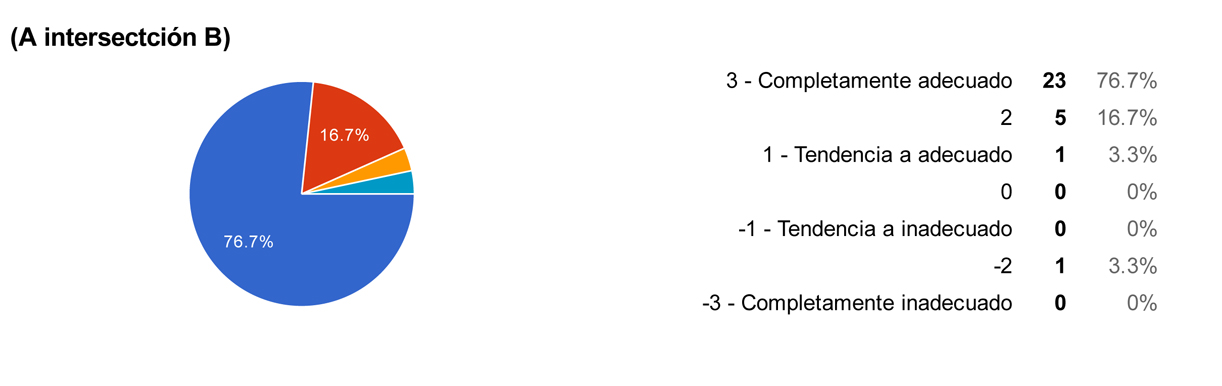
\includegraphics[width=15cm, height=4.74cm]{Figures/hjudgement/r8}
	\caption[]{}
\label{fig:parsed_corpus}
\end{figure}

\begin{figure}[H]
\centering
	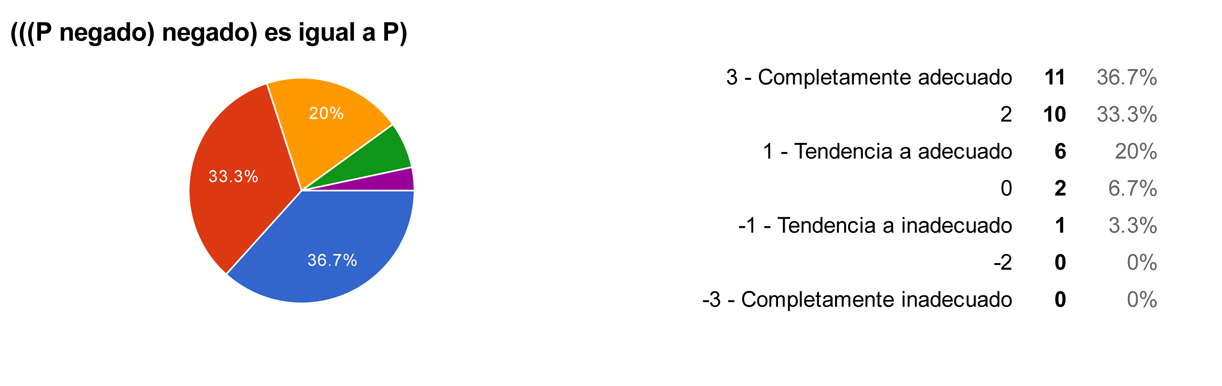
\includegraphics[width=15cm, height=4.74cm]{Figures/hjudgement/r9}
	\caption[]{}
\label{fig:parsed_corpus}
\end{figure}

\begin{figure}[H]
\centering
	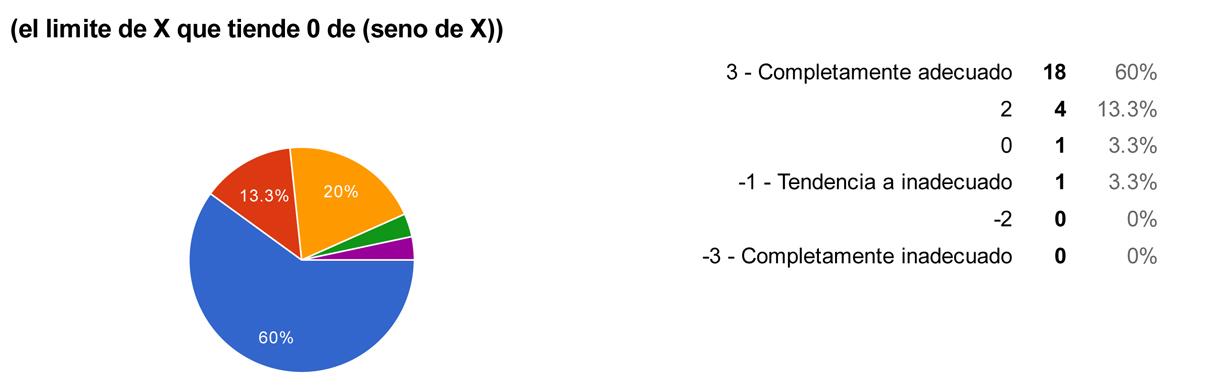
\includegraphics[width=15cm, height=4.74cm]{Figures/hjudgement/r10}
	\caption[]{}
\label{fig:parsed_corpus}
\end{figure}

\begin{figure}[H]
\centering
	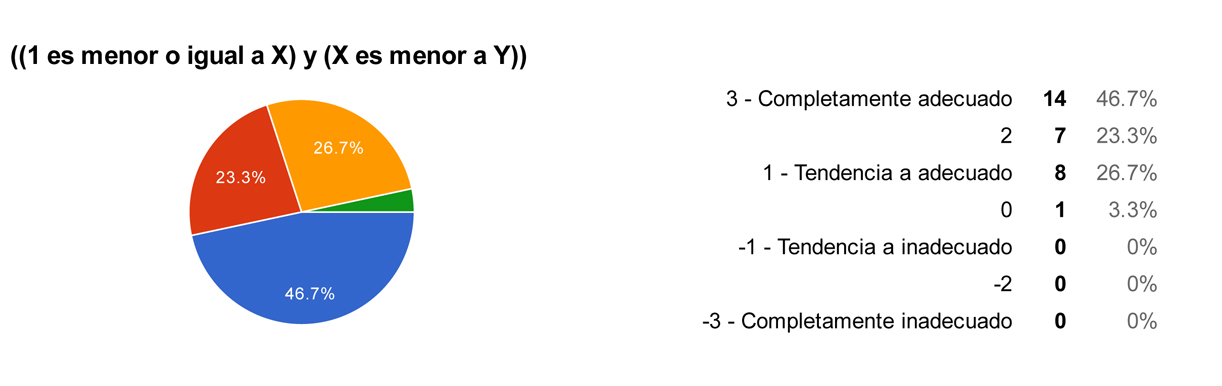
\includegraphics[width=15cm, height=4.74cm]{Figures/hjudgement/r11}
	\caption[]{}
\label{fig:parsed_corpus}
\end{figure}

\begin{figure}[H]
\centering
	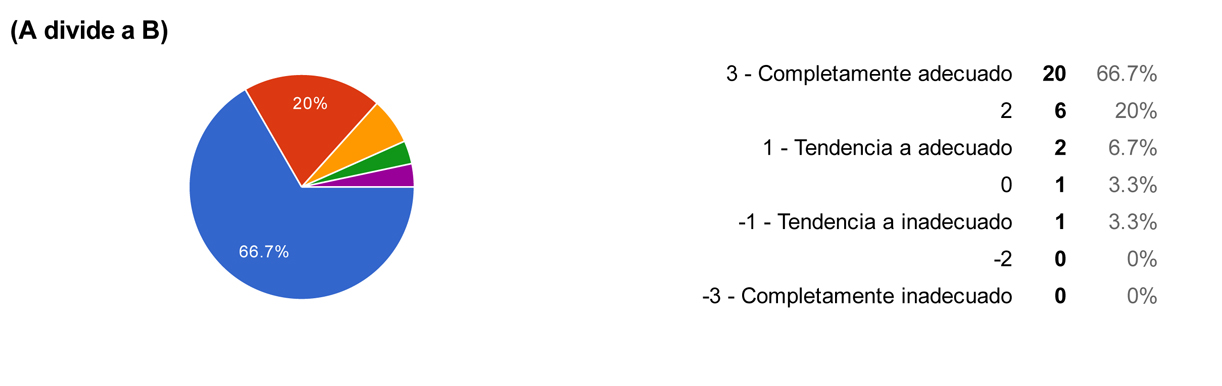
\includegraphics[width=15cm, height=4.74cm]{Figures/hjudgement/r12}
	\caption[]{}
\label{fig:parsed_corpus}
\end{figure}

\begin{figure}[H]
\centering
	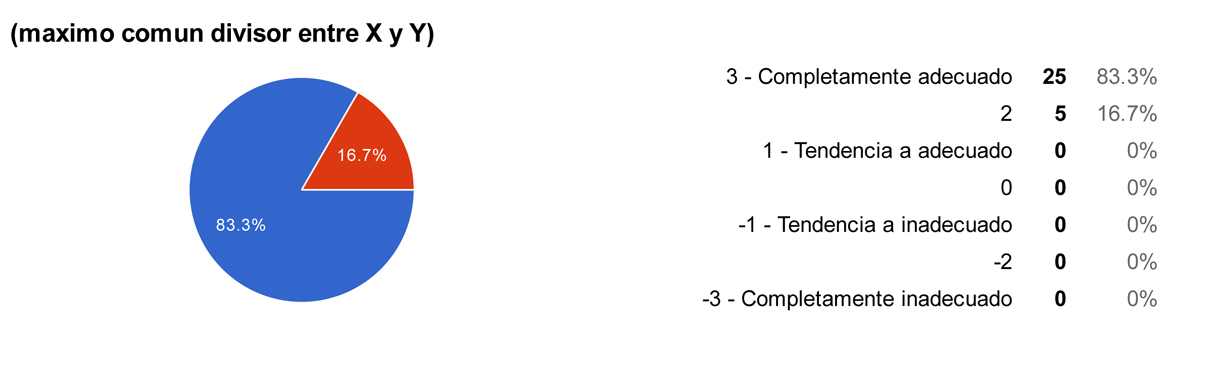
\includegraphics[width=15cm, height=4.74cm]{Figures/hjudgement/r13}
	\caption[]{}
\label{fig:parsed_corpus}
\end{figure}

\begin{figure}[H]
\centering
	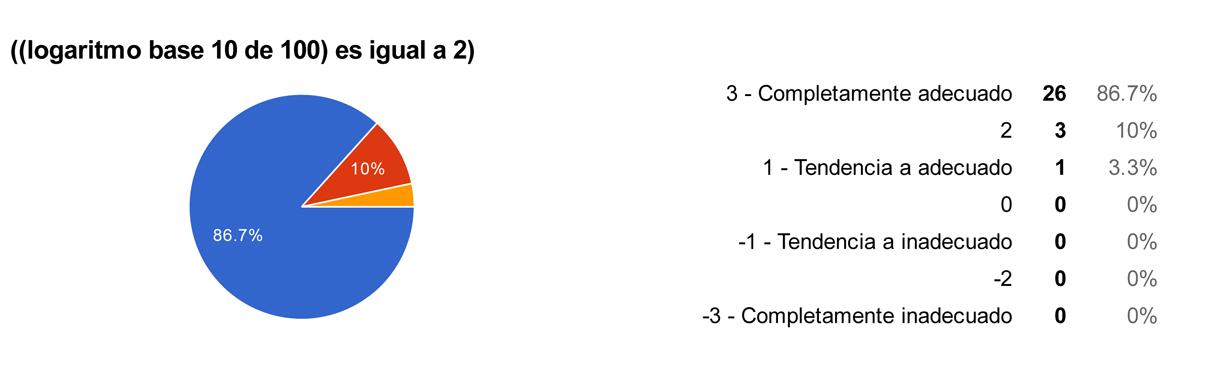
\includegraphics[width=15cm, height=4.74cm]{Figures/hjudgement/r14}
	\caption[]{}
\label{fig:parsed_corpus}
\end{figure}

\begin{figure}[H]
\centering
	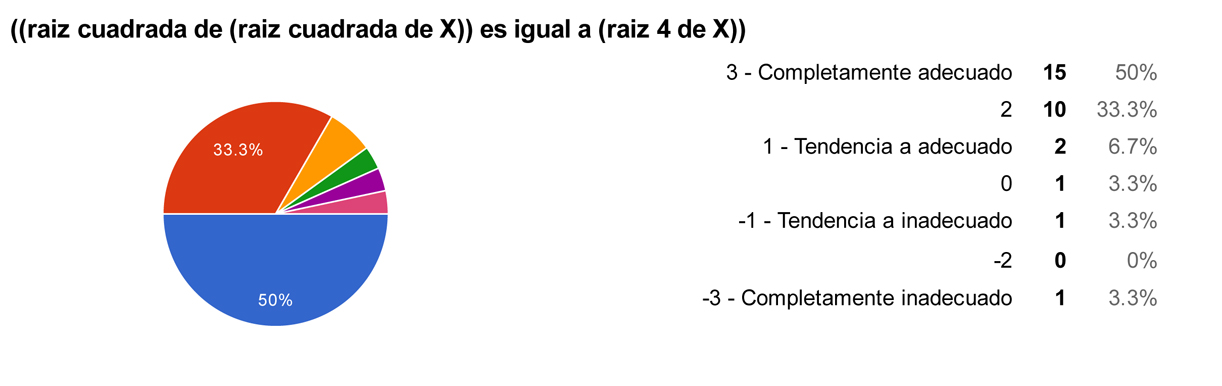
\includegraphics[width=15cm, height=4.74cm]{Figures/hjudgement/r15}
	\caption[]{}
\label{fig:parsed_corpus}
\end{figure}

\begin{figure}[H]
\centering
	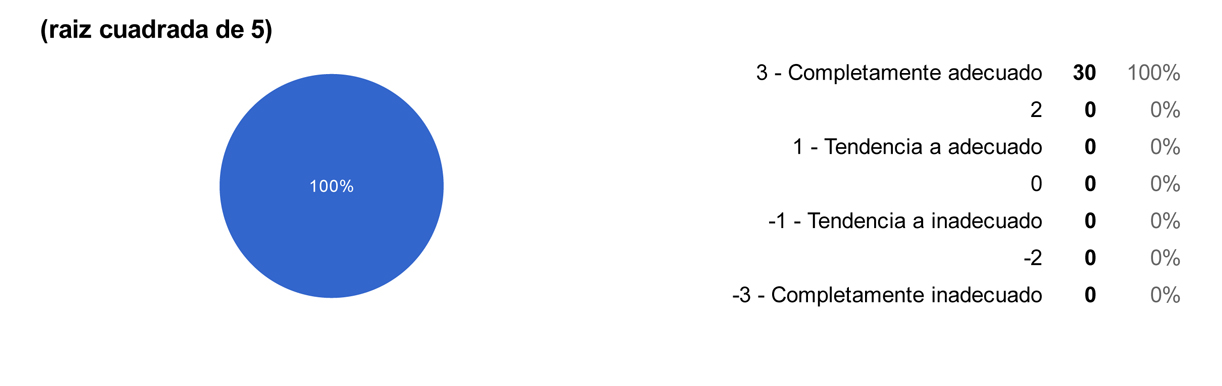
\includegraphics[width=15cm, height=4.74cm]{Figures/hjudgement/r16}
	\caption[]{}
\label{fig:parsed_corpus}
\end{figure}

\begin{figure}[H]
\centering
	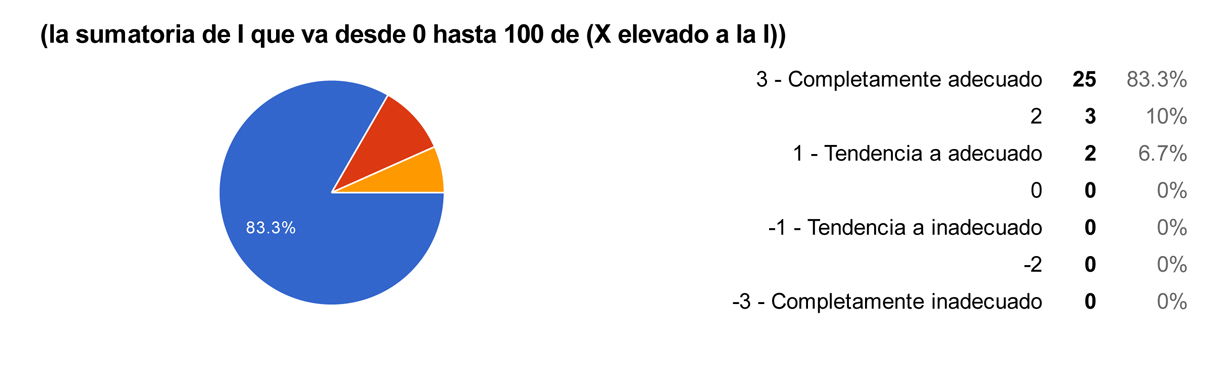
\includegraphics[width=15cm, height=4.74cm]{Figures/hjudgement/r17}
	\caption[]{}
\label{fig:parsed_corpus}
\end{figure}

\begin{figure}[H]
\centering
	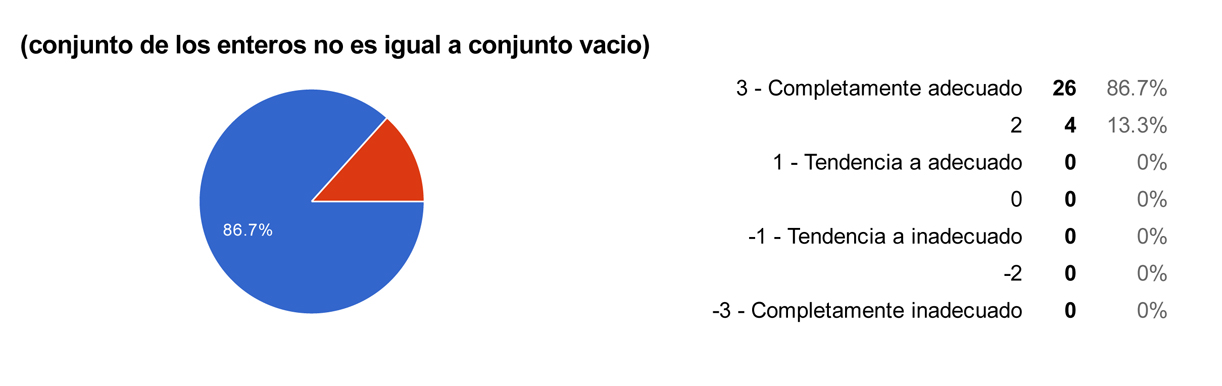
\includegraphics[width=15cm, height=4.74cm]{Figures/hjudgement/r18}
	\caption[]{}
\label{fig:parsed_corpus}
\end{figure}

\begin{figure}[H]
\centering
	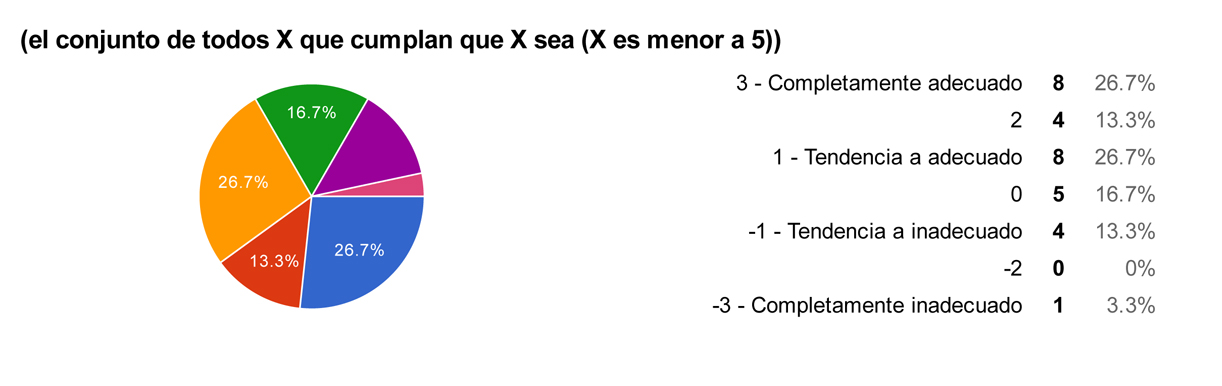
\includegraphics[width=15cm, height=4.74cm]{Figures/hjudgement/r19}
	\caption[]{}
\label{fig:parsed_corpus}
\end{figure}

